\section{Proposed Work}
\subsection{Implementation}

% unsupervised anomaly score
The project will solve PdM hurdles for operators in modernized workplaces by providing an accurate estimate of asset health.
The proposed method is to replicate the results achieved by other papers using SOMs for condition monitoring. 
Specifically, to train a SOM and get a health score by calculating how much a test data point deviates from normal operation.
The higher the health score, the lower the operating condition of the asset.
Various SOM implementations will be examined, such as the \href{https://pypi.org/project/kohonen/}{Kohenen 1.1.2 Python package} (documentation for this package is sparse).
If these do not provide enough customization then a SOM will be self-coded using Tensorflow.
Customization may be required to allow the comparison of various distance metrics to get a health score.
As discussed, this has been done before but is rarely seen in industry today.
The use of these algorithms on real and significant data is challenging and relevant.
For example, the data will be provided in hourly chunks throughout the year (instead of one continuous dataset).
Futhermore, pre and post processing techniques will be explored to improve performance, useability and interpretability.
Decision boundaries will be learned as a final step (if we have enough failure data) to organize failures into different classes and severity levels.

\begin{figure}[!h]
    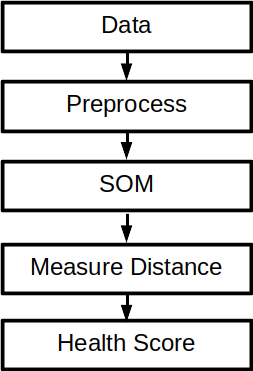
\includegraphics[width=3cm]{steps}
    \centering
    \label{fig:steps}
    \caption{Implementation steps from Data.}
\end{figure}

\subsection{Evaluation}

An expected significant challenge will be the model's ability to generalize, given that the datasets span only a days worth of operation in total.
To avoid overfitting, the number of dimensions will be kept low and regularization will be used where possible.
To judge the models ability to generalize and to evaluate performance, the algorithm will be tested on two datasets: unhealthy operation (1) and healthy operation (2).
Precision was chosen as a metric for (2) to minimize the number of false positives.
This is especially important because this is an experimental project with the steel manufacturer, so it is important that the algorithm does not do more harm than good.
For (1), the algorithm should produce a value indicative of failure at least 75\% of the time.


Performance evaluation of the algorithm from a PdM context will be performed against each of these three scenarios.
\begin{enumerate}
    \item Run-to-Failure: how will the proposed solution compare if no maintenance is performed?
    \item Preventative: how will the proposed solution compare if PvM is performed (the current process of the plant)?
    \item Other Predictive Methods: how will the proposed solution compare if another PdM solution is performed?
\end{enumerate}

Other metrcs for evaluation will include the following: cost, latency (time between failure and an indication of failure from the algorithm) and training time.
Finally, the algorithm will also be scrunitized by a subject matter expert (SME) in terms of usability and interpretability.


\subsection{Timeline}

The time from the proposal submission date and the final due date is six weeks.

\begin{enumerate}
	\item Week 1: Choose a SOM algorithm or develop one.
    \item Week 2: Choose a SOM algorithm or develop one.
    \item Week 3: Test algorithm on data, visualize.
    \item Week 4: Choose and evaluate various distance metrics.
    \item Week 5: Tune model, test, repeat. Try preprocessing methods.
    \item Week 6: Report writing and final touchups.
\end{enumerate}